\documentclass[2pt]{report}
\input{preamble.tex}
\usepackage[scr]{rsfso}

\newcommand{\faketarget}{\oplus\!\!\!\!\odot}
\newcommand{\target}{%
  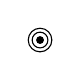
\begin{tikzpicture}[scale=0.5]
    \fill[black] (0,0) circle (0.1);
    \draw (0,0) circle (0.2);
    \draw (0,0) circle (0.3);
  \end{tikzpicture}%
}

\usepackage[clock]{ifsym}


\title{\Huge{Interface Personne Marchine}\\{IFT2905}\\{\textbf{Introduction}}}
\author{\huge{Franz Girardin}}
\date{\today}
\lstset{inputencoding=utf8/latin1}

            %%%%%%%%%%%%%%%%%  Sect.                          %%%%%%%%%%%%%%%%%%%%%%%%%%%%%%%%%%%%%%%%%%%%%%%%%%%%%%%%%
\usepackage{helvet}
\titleformat{\chapter}
  {\fontfamily{phv}\bfseries\huge} % format
  {}                % label
  {0pt}             % sep
  {\color{myb}\huge}           % before-code



\titleformat{\section}
  {\normalfont\scshape}{\thesection}{1em}{}


% Customizing the spacing for the chapter titles
\titlespacing*{\chapter}{0pt}{0pt}{20pt}

\usepackage[utopia]{mathdesign}
% Allow hfill in math environment
\newcommand{\specialcell}[1]{\ifmeasuring@#1\else\omit$\displaystyle#1$\ignorespaces\fi}

% Allow you to do the non implication (implication barred)
\newcommand{\notimplies}{%
  \mathrel{{\ooalign{\hidewidth$\not\phantom{=}$\hidewidth\cr$\implies$}}}}



\DeclareRobustCommand{\looongrightarrow}{%
  \DOTSB\relbar\joinrel\relbar\joinrel\relbar\joinrel\rightarrow
}

\begin{document}
\maketitle

\pagebreak

\pagebreak
\begin{multicols*}{3}


    \footnotesize


    \paragraph{Mythe de l'erreur humaine} $\mathcal{H}$   
    Les \textit{échecs} d'un système $\mathbb{PM}$ sont souvent dus  
    au \textbf{design}. Pour $\downarrow$ erreur $\mathcal{H}$ : 
    \begin{itemize}
        \item[$\rhd$ ] Design qui tient compte des \textbf{limitations}
            et de la \textbf{fiabilité} des $\mathcal{H}$.   
    \end{itemize}

    \paragraph{Principes de design}
    \begin{itemize}
        \item[$\rhd$] Utilisabilité
        \item[$\rhd$] Expérience de l'Utilisateur ($\mathbb{UX}$)
        \item[$\rhd$] \textbf{Psychopathologie} : frustratiosn courantes  
         \item[$\blacktriangleright$] Permettent de 
             \textbf{critiquer}, \textbf{analyser} et \textbf{convervoir} interfaces.     

    \end{itemize}


    \paragraph{Causes d'échecs}
    \begin{itemize}
        \item[$\rhd$] Fonctionnalité 
            \begin{itemize}
                \item[$\blacktriangleright$] $\mathcal{U}$ ne connait pas fonctions de l'objet
                \item[$\blacktriangleright$] L'objet ne fait pas ce que  
                    $\mathcal{U}$ désire. 
            \end{itemize}
        \item[$\rhd$] Visibilité 
            \begin{itemize}
                \item[$\blacktriangleright$] $\mathcal{U}$ ne \textbf{voit} 
                    pas certaines infos de l'objet   
                \item[$\blacktriangleright$] 
                    $\mathcal{U}$ ne sait pas quelle séquence de contrôle est nécessaire pour 
                    atteindre son but.  
                \item[$\rhd$] E.g. Lumières enfoncée pour passage piétons
            \end{itemize}
        \item[$\rhd$] Feedback 
            \begin{itemize}
                \item[$\blacktriangleright$] Comment $\mathcal{U}$ 
                    sait si les opérations ont réussi ?
                \item[$\blacktriangleright$] 
                    Comment $\mathcal{U}$ 
                    sait s'il y a une erreur en cours de route ?
            \end{itemize}
    \end{itemize}

    \paragraph{Buts du $\mathbb{UX}$ | }
    $\mathbb{MAUSSEE}$ : $\mathbb{M}$émorabilité, 
    $\mathbb{A}$pprentissage, $\mathbb{U}$tilité,
    $\mathbb{S}$écurité, $\mathbb{S}$atisfaction, 
    $\mathbb{E}$fficience, $\mathbb{E}$fficacité. 

    \paragraph{Définition de l'utilisabilité}
    Degré selon lequel un produit peut être utilisé par des 
    $\mathcal{U}$ \textit{identifiés}, pour atteindre des 
    \textbf{buts} \textit{définis} par 
    l\textbf{'efficacité}, l\textbf{'efficience} et 
    la \textbf{satisfaction}.   
    \begin{itemize}
        \item [$\rhd$] \textbf{ Efficacité} : atteindre le but \;  $\target$
        \item[$\rhd$] \textbf{ Efficience} : \textit{effort} 
            et ou \textit{temps} \textbf{minimal} \; \showclock{0}{45} 
        \item[$\rhd $] \textbf{ Satisfaction} :  
            évaluation subjective par $\mathcal{U}$
    \end{itemize}

    \paragraph{Où les desginer se trompent}  
    \begin{itemize}
        \item[$\rhd$] Ne comprennet pas $\mathcal{U}$ et leurs limitations
        \item[$\rhd$] Ne prévoient pas différents \textbf{contextes d'utilisation}  
        \item[$\rhd$] Absence de \textbf{modèle détaillé} du fonct.        
        \item[$\rhd$] Absence de \textbf{feedback} par l'objet.        
    \end{itemize}

    \paragraph{Pourquoi le design est-il difficile}
    Les \textbf{interactions} sont complexes et difficile à définir. Par ailleurs, les tâches 
    sont complexes et \textit{implicites}. Il faut distribuer \textit{raisonnablement}
    les tâches à la machine et à l'$\mathcal{U}$ pour éviter que l'un ou l'autre 
    ne soit pas confronté à une complexité excessive. 

    \paragraph{Principe de découvrabilité}
    L'$\mathcal{U}$ doit savoir immédiatement à quoi l'objet sert, comment 
    l'utiliser et quelles sont les opérations possibles. 

    \begin{itemize}
        \item[$\rhd$]  \textbf{Affordance} ce que l'O permet de faire.  
            Un \textit{signifiant} est un élément qui permet de rendre 
            \textbf{l'affordance} visible.   
        \item[$\rhd$]  \textbf{Signifiants} indiquent que l'affordance 
            $\exists$ et ne doivent pas être \textbf{contradictoire}.   

        \item[$\rhd$]  \textbf{Anti-affordance} permettent de masquer 
            visibilité d'un aff. et contribue à la gestion d'erreur. 

        \item[$\rhd$]   \textbf{Correspondance} Permet de faire 
            l'association lors de l'utilisation 
            (direction volume, mode \texttt{on}/\texttt{off})
    \end{itemize} 



    \end{multicols*}


\end{document}
